\section{Demonstrating Improved Accuracy}
\label{sec:accuracy}

Now comes the time to justify our efforts by comparing the accuracy of our
skew-normal approximation to that of the normal.

\subsection{Visual Comparison}

The first and most obvious way of judging accuracy is by visual inspection.
Figures \ref{fig:comparison-n25}, \ref{fig:comparison-n50}, and
\ref{fig:comparison-n100} compare the binomial, normal, and skew-normal at
small values of $p$ for $n=25$, $n=50$, and $n=100$, respectively. It is not
hard to see that, especially at very small $n$ and $p$, our skew-normal curve
follows the shape of the binomial much more closely.

\begin{figure}
  \centering
  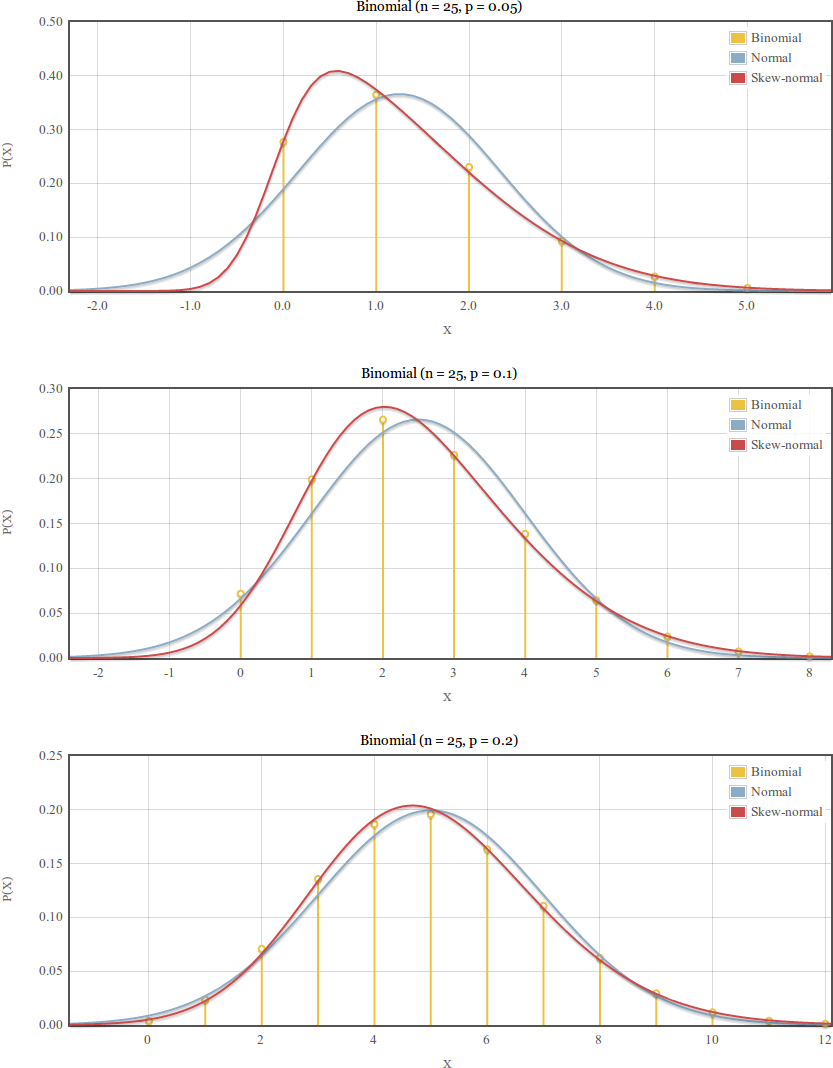
\includegraphics[width=\textwidth]{../images/comparison-n25.png}
  \caption{Binomial, normal, and skew-normal, $n=25$}
  \label{fig:comparison-n25}
\end{figure}

\begin{figure}
  \centering
  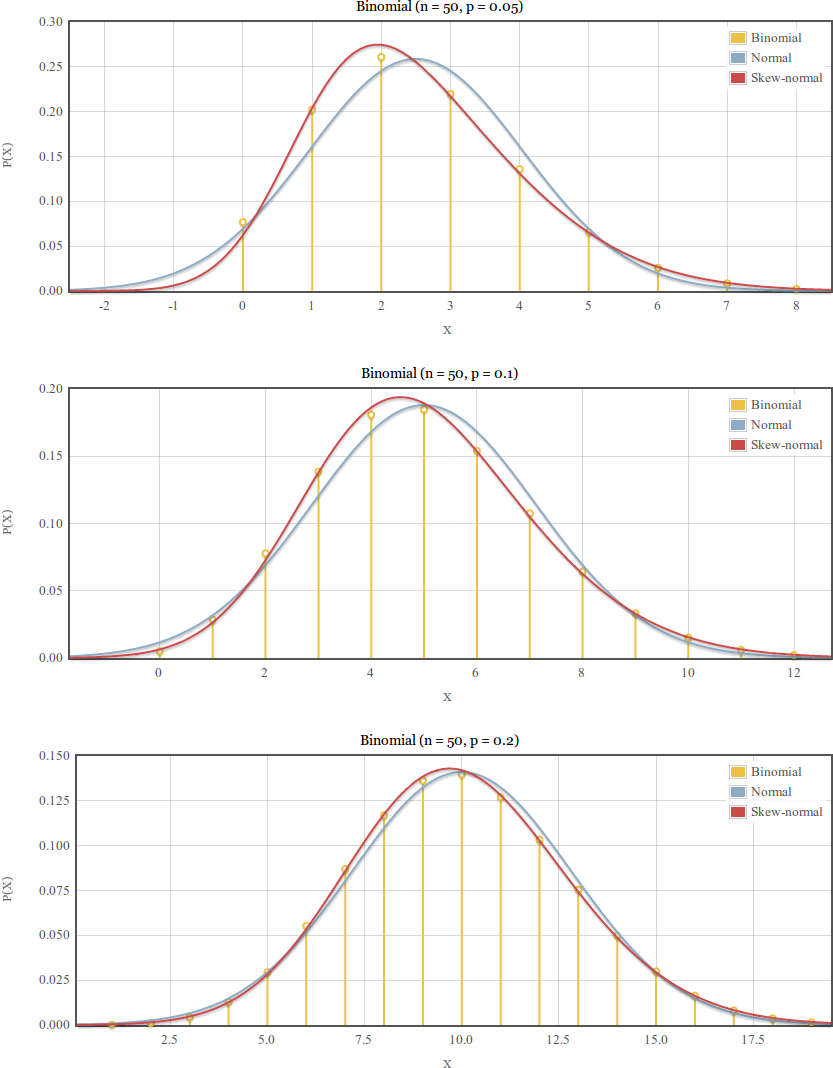
\includegraphics[width=\textwidth]{../images/comparison-n50.png}
  \caption{Binomial, normal, and skew-normal, $n=50$}
  \label{fig:comparison-n50}
\end{figure}

\begin{figure}
  \centering
  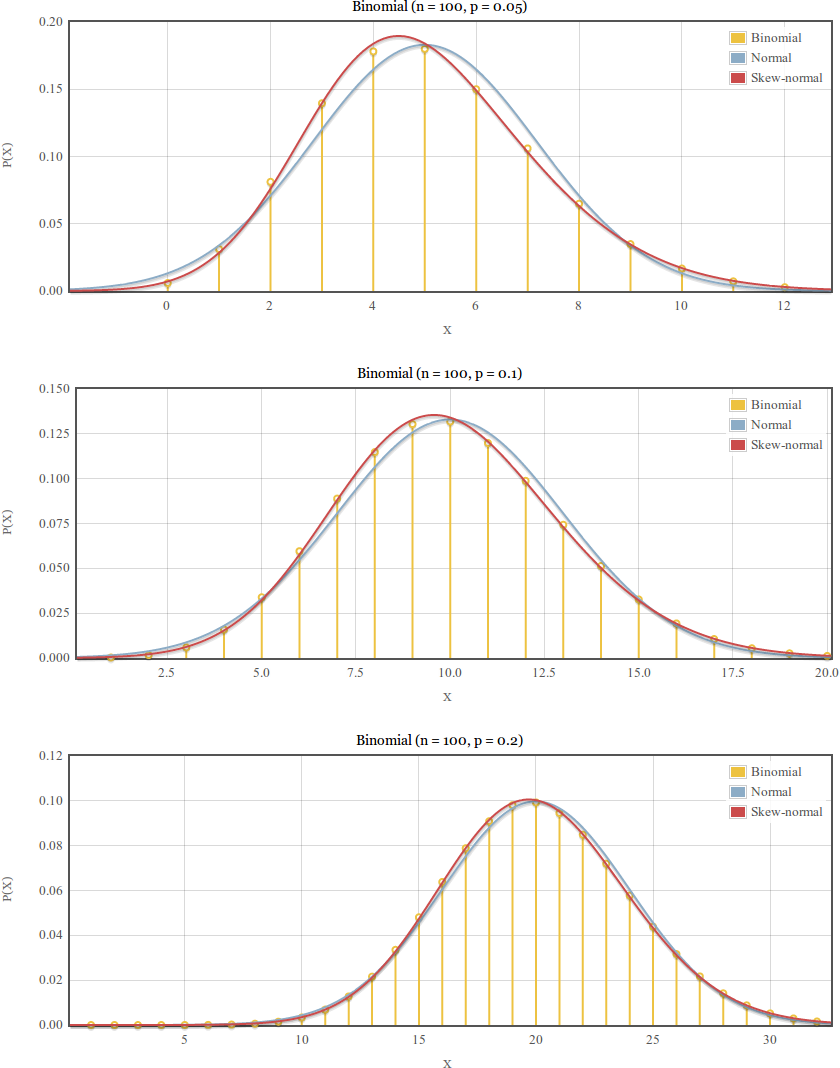
\includegraphics[width=\textwidth]{../images/comparison-n100.png}
  \caption{Binomial, normal, and skew-normal, $n=100$}
  \label{fig:comparison-n100}
\end{figure}

\subsection{Maximal Absolute Error}
\label{subsec:mabs}

A quantitative method of judging accuracy is comparing the maximal absolute
errors of our two approximations, defined by \citet{mabs} as

\begin{equation}
  \textnormal{MABS}(n, p) \eq \max_{k \in \{0, 1,...,n\}} \left| F_{B(n,p)} (k) -  F_{\textnormal{appr}(n,p)}(k + 0.5) \right|
\end{equation}

where $F_{B(n,p)}$ is the cdf of the binomial and $F_{\textnormal{appr}(n,p)}$
is the cdf of either the normal or skew-normal approximation; the 0.5 is a
continuity correction.

Figures \ref{fig:mabs-fixed-n} and \ref{fig:mabs-fixed-p} shows the MABS of the
skew-normal and normal approximations as a function of $p$ and $n$,
respectively. Again, the skew-normal outperforms the normal considerably in the
extreme ranges, with the two approximations converging as $n \rightarrow
\infty$ or $p \rightarrow 0.5$.

\begin{figure}
  \centering
  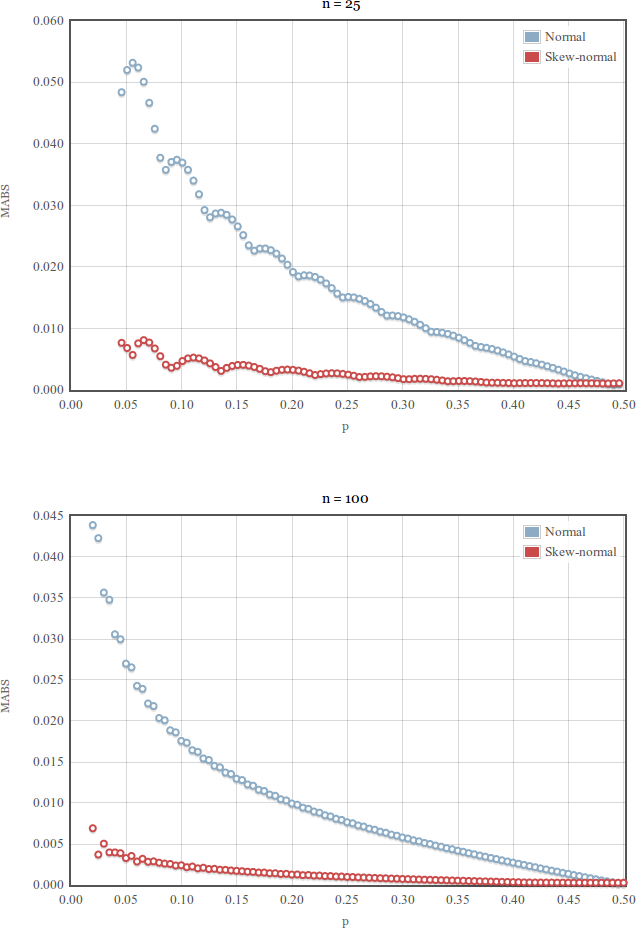
\includegraphics[width=\textwidth]{../images/mabs-fixed-n.png}
  \caption{MABS as a function of p}
  \label{fig:mabs-fixed-n}
\end{figure}

\begin{figure}
  \centering
  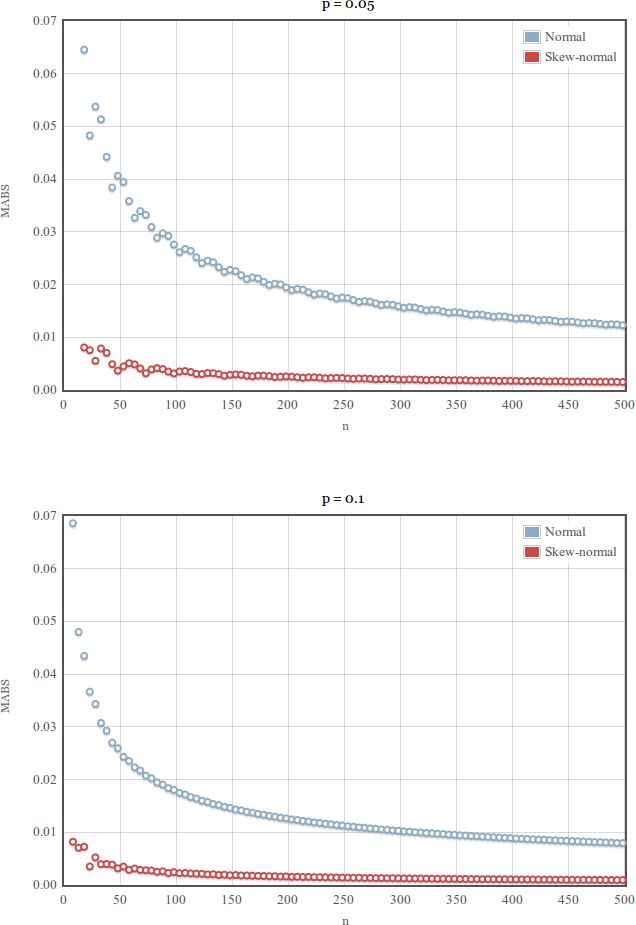
\includegraphics[width=\textwidth]{../images/mabs-fixed-p.png}
  \caption{MABS as a function of n}
  \label{fig:mabs-fixed-p}
\end{figure}

\clearpage
